\documentclass{article}
\usepackage{graphicx}
%DIF PREAMBLE EXTENSION ADDED BY LATEXDIFF
%DIF UNDERLINE PREAMBLE %DIF PREAMBLE
\RequirePackage[normalem]{ulem} %DIF PREAMBLE
\RequirePackage{color}\definecolor{RED}{rgb}{1,0,0}\definecolor{BLUE}{rgb}{0,0,1} %DIF PREAMBLE
\providecommand{\DIFadd}[1]{{\protect\color{blue}\uwave{#1}}} %DIF PREAMBLE
\providecommand{\DIFdel}[1]{{\protect\color{red}\sout{#1}}}                      %DIF PREAMBLE
%DIF SAFE PREAMBLE %DIF PREAMBLE
\providecommand{\DIFaddbegin}{} %DIF PREAMBLE
\providecommand{\DIFaddend}{} %DIF PREAMBLE
\providecommand{\DIFdelbegin}{} %DIF PREAMBLE
\providecommand{\DIFdelend}{} %DIF PREAMBLE
%DIF FLOATSAFE PREAMBLE %DIF PREAMBLE
\providecommand{\DIFaddFL}[1]{\DIFadd{#1}} %DIF PREAMBLE
\providecommand{\DIFdelFL}[1]{\DIFdel{#1}} %DIF PREAMBLE
\providecommand{\DIFaddbeginFL}{} %DIF PREAMBLE
\providecommand{\DIFaddendFL}{} %DIF PREAMBLE
\providecommand{\DIFdelbeginFL}{} %DIF PREAMBLE
\providecommand{\DIFdelendFL}{} %DIF PREAMBLE
%DIF END PREAMBLE EXTENSION ADDED BY LATEXDIFF

\begin{document}


\title{E-Lab: Web based platform for solving and automatic assessment of
programming problems}

\author{Tomche Delev}

\maketitle

\begin{abstract}

\emph{E-Lab} is a platform developed at Faculty of Computer Science and
Engineering for solving and auto-grading programming problems from introduction
programming courses. The main goal is to simplify, organize and
improve the process of solving programming problems from large group of
students in dedicated computer labs using centralized server for compiling and saving their
work. All the work from the students can be done in a web browser using the
web-based code editor and everything is stored on the server file system.
All the problems and solutions are under version control system (Git). The
platform supports different types of problems in several programming languages
(C, C++, Java) and it's designed in a manner so it can be easily extended. \DIFaddbegin \DIFadd{Here
we add some text.
}\DIFaddend \end{abstract}

\section{Introduction}
Programming is one of the essential practical skills tought at introduction
level courses in computer science curiculums. Mastering this skill can gain the
students good chances of finding good job and developing successfull career. The
rewarding career and the constant rising of the market for programmers \DIFdelbegin \DIFdel{makes }\DIFdelend \DIFaddbegin \DIFadd{defines
}\DIFaddend the computer science programs very popular among high school students. The results
are large introduction classes with several hundred students enrolled. 

Programming is not an easy skill to devolop. By some studies
\cite{winslow1996programming} mastering this skill requires up to ten years. As
easy as it seems teaching basic programming rises challenges to the academic
stuff and good organisation with the right tools is required to tackle theese
challenges. \DIFdelbegin \DIFdel{Similary to other practical skills, good }\DIFdelend \DIFaddbegin \DIFadd{Good }\DIFaddend strategy for learning
programming involves great amount of time actually doing it. In introduction
level courses involinvg some kind of programming, this translates to solving a
lot of basic algorithmic examples. One third of the time teaching these courses
is dedicated to solving this kind of programming problems organized in problem sets by the
topic and executed in dedicated computer labs.

Several hundered students working on problems every week produces thousends
solutions in form of source code that should be examined and graded. In the
current environment students work on PC workstations using simple text
editor or some kind of IDE for the programming language they use. They save,
compile and execute the solutions on their local machines. After they finish, no
records of their work is stored on server repository, so there is no
possibility for the instructors to examine and grade their solutions afterwards.
The time limit for each group of students is in the range of 90 to 120 minutes,
and the instructors usually have only up to 30 minutes to examine, test and
grade 20 students, each with several solutions. These settings makes almost
impossible for the instructors to quality assess the students work.

The nature of the programming problems in great part of the introduction
programming courses is algorithmic. This makes it possible to develop a fairly
simple platform for creating problems, test cases and system for automatic
assessment and grading of the solutions. Most algorithmic problems can be
designed to take some input from the standard input in some prescribed format,
apply some simple algorithm in memory on this input, and finally produce an
output in some prescribed format and print it on the standard output. Having
this kind of problems we can take the executable of the program, feed the
test input and then compare and verify for correctnes on the test output. This
process which is widely used in many competitive programming systems, should
emphasize the importance in programming to have a working solutions, instead of only
writing a code that some times even doesn't compile.

The E-Lab system is developed with many goals. If the first goal was to better
handle the organization and implementation of the programming exercises, other
important goals are the motivation of the students and the continous feedback
they will have using this platform. With E-Lab we want to shift the role of the
instructors from teachers and graders to motivators, which is shown to give
better effects in teaching programming \cite{jenkins2001teaching}.

\section{Related work}

Systems that automatically assess programming assignments have been designed and
used for more than fourty years. In \cite{douce2005automatic} authors review
a number of the influential systems for automatic test-based assessment
of programming asignments. These systems are broadly categorized according to
age in three generations. 

The first generation or early assessment systems were
those orginate from the time when programming was done using punch cards and the
evaluation was done by executing this problems and manually evaluating the
output. Some of these early systems had specially designed programms to
compare the output of the programm to some predefined output. 

The second generation or the tool oriented assessment systems are developed
using pre-existing tool sets and utilities supplied with the operating system or
programming environment. One notable example of these systems is the BOSS
system originated at the University of Warwick in the UK \cite{joy2005boss} which in
his last development cycles has become an assessment management system. Other
example is the Scheme-Robo project \cite{saikkonen2001fully} which has been
supplemented by a graphical user interface and an algorithm-animation component.

The third-generation assesment system are characterized by using the latest
developments in web technology and adopt advanced testing approaches. Previously
mentioned system BOSS has evolved in this generation. CourseMarker, developed at
Nottingham University \cite{higgins2003coursemarker} and RoboProf deployed at
Dublin City University \cite{daly2004automated} are examples of this last
generation of automatic assessment systems.

\section{The E-Lab philosophy}

We developed E-Lab with the idea that we should build using the latest web
technologies and state of the art tools that have been proven to work over the
years. The result is a forth generation system, where we integrate latest
technologies to produce modern, extendable, scalable and easy to use platform.
We achieve this using the experince over the years observing students working on
programming problems in introduction level courses. 

\subsection{Integrated problem view}

Most of the time available to students trying to solve the problems in the
dedicated computer labs is or should be spent in three equally important phases.
In the first phase students should carefully read and understand the problems,
the second phase should be the coding part in which they can refere to the
related course material, and in the third and final phase they should get the
feedback for the corectness of their solution.

\begin{figure}
\centering
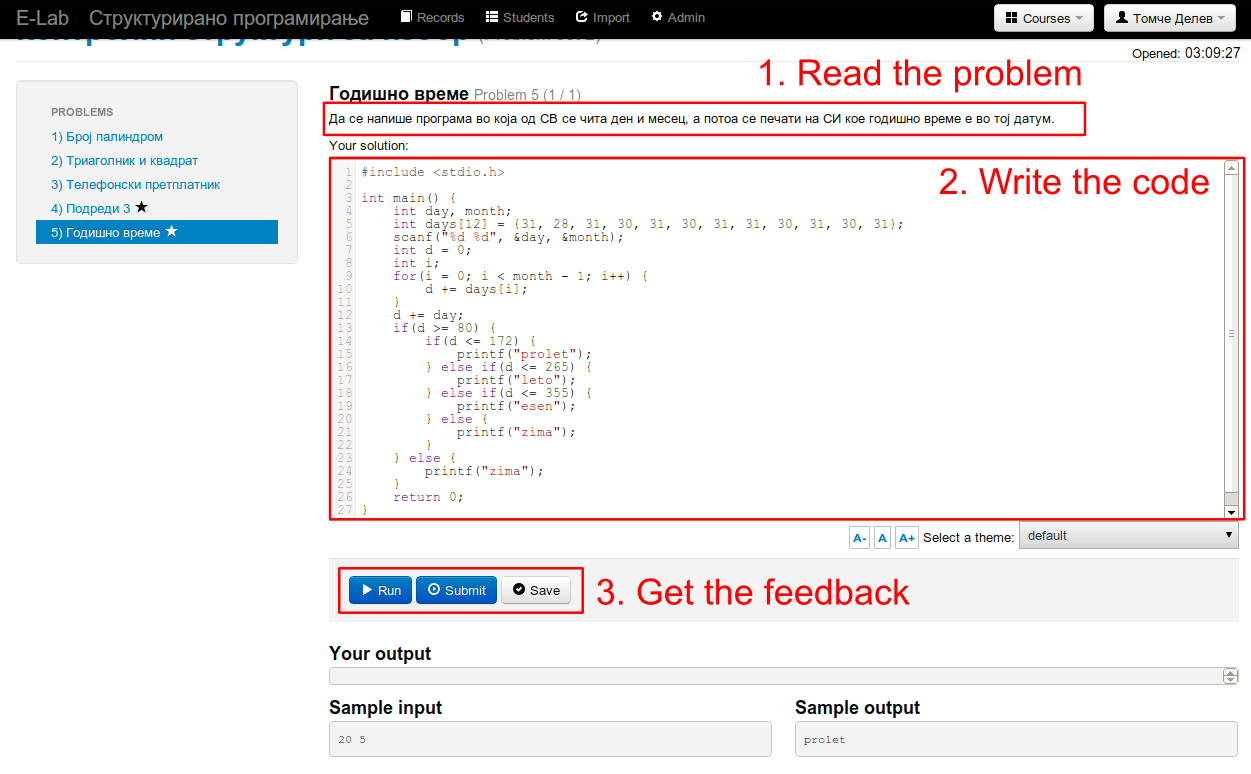
\includegraphics[width=.99\textwidth]{e-lab/user_screen}
\caption{The student screen trying to solve a problem.}
\label{fig:student_screen}
\end{figure}

According to this observation, the platform was designed so that on single
screen students can work and acomplish all the phases involved in solving the
problems. As can be seen on figure \ref{fig:student_screen}, on a single screen
we have the problem text to be read, the web-based code editor to write the
solution and the actions pane, so they can run their solution and get instant
feedback in the ouptut area. With this design we try to implement the extreme
apprenticeship method \cite{vihavainen2011extreme} which is based on a set of
values and practices that emphasize learning by doing together with continuous
feedback as the most efficient means for learning programming.

\subsection{Authentication}
All users of the system are authenticated using the Central Authentication
System (CAS) which is used by all services at the faculty. With this mechanism
we can identify students and their solutions, and later use this identity to
check for plagiarism, malicious code or other abusive usages. 

\subsection{Problems design}
The central entity in the programming exsercises are the programming problems.
Each problem is designed in two phases. In the first phase we define the problem
text, name and in some problems provide starter code. This information define
only the basis of the problem, so in the second phase we need to provide sample
input and output for the problem as an example, and at least one test case also
in form of input and output data so the solutions of the problem can be tested.
For each problem we can also add contextual help or hints that can be helpful
for students to solve the problem.

\subsection{Problems and solutions repository}
Almost all of the problems information and solutions are in form of simple text
or source code files. Very practial way of storing this kind of data is using
some kind of version control system. With this system we get features such as
management of the changes of the documents and full revision tracking
capabilities. The choice of Git, which is very fast distributed revision control
system, gives the system the reliability of the distributed repositories that
doesn't deppend on single server.

\subsection{Sandboxed execution}
The system allows students to write, run and execute any kind of program code
that will be executed on a remote server. This can harm the server in many
undesirable ways. The malicious code can contain unprivileged read and write
access, can create process bombs, allocate all the availble memory or simply
consume all the processing power available to the server. To control or prevent
these security issues all the execution is done in sandbox environment. In this
sandbox each execution is limited by processing time and memory, and also
constrained in the number of processes it can fork.

chroot
ulimit

\subsection{Automatic assesment}
Having limited resourses in time and the actual inability to assess all of the
student solutions to the provided problems makes the automatic assessment
top priority in the platform. Since the platform covers only introduction level
courses in programming and algorithms, most of the problems can be designed so
they can be assessed by simple black-box testing methodology. For each problem
the author provides a reference solution, and using this solution the system
generates test cases. Each test case consists of simple input and output text
files. So when tested the compiled programm feeded the input file to be correct
should output the same output as the contents in the generated output file. One
of the test cases is the sample test case which is visible for the students so
they can better understand the problem. Each problem should have at least one
test case and up to ten test cases. We limit the number of test cases, to be
able to provide instant feedback


\section{Architecture}

\begin{figure}
\centering
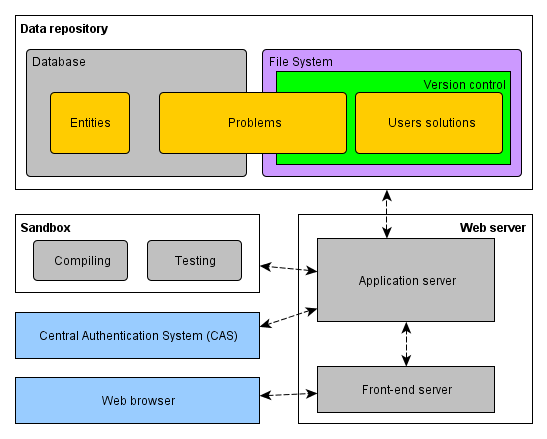
\includegraphics[width=.99\textwidth]{e-lab/architecture}
\caption{The E-Lab architecture.}
\label{fig:architecture}
\end{figure}

The overview of the platform architecture can be seen on figure
\ref{fig:architecture}, showing it's primary components. The data repository
is the most interesting component of the system. We propose a specific way of
storing the problems and all the work from the students by using a combination
of database and file system. All the relational data and metadata of the
problems such as the name, the problem set it belongs, the text is stored in
relational database. The other part containing a the starter code, reference
solution, help contents in markup language and all the test cases in form of
input and output text files are stored on the file system. Also, all of the
students solutions are stored solely on the file system in organized directory
structure.

\subsection{The client-server}

The system is a form of a standard client-server web architecture. This
architectures allows the client, which is standard and web browser available on
all platforms, to run on virtually every PC in our computer lab environment.
This lowers the costs of maintainence of the computer labs, because no specific
software such as separate client software, compilers, IDEs or text editors
should be installed and maintained.

The web server is composed of two separate servers. The front-end web server is
a fast web server that serves as a fast proxy and load balancer to the
application server. The application server is Java server that uses a scalable
RESTfull architecture. The web applications on this server follows the MVC
architectural pattern applied to the web architecture.
The authentication of the users is done on a central authentication server using
HTTPS. 

\section{Detecting plagiarism}

\section{Conclusion}

\bibliographystyle{ieeetr}

\bibliography{e-lab}

\end{document}

